\IEEEraisesectionheading{\section{Introduction}\label{sec:introduction}}


Humans are faced with a stream of high-dimensional sensory inputs and minimal external supervision, and yet, remarkably, are able to learn a range of complex yet generalizable concepts and behaviors.
While there has been significant progress in developing deep reinforcement learning algorithms that learn complex skills~\cite{tdgammon,alphago,openai_hand} and scale to high-dimensional observation spaces, such as pixels~\cite{atari,e2e}, learning behaviors that \emph{generalize} to new objects, goals, or environments remains an open problem.
The key to generalization is diversity -- when deployed in a narrow, closed-world environment, a reinforcement learning algorithm will recover skills that are successful only in a narrow range of settings. 
However, the problem of learning skills in diverse, open-world environments, such as the real world, presents a number of significant challenges: external reward feedback is extremely sparse, if existent at all, and the agent has only indirect control over the environment and indirect access to the state of the environment -- through its senses.

We approach this problem from the standpoint of sensory prediction. Prediction is often considered a fundamental component of intelligence, and, crucially, prediction of raw sensory observations does not make any assumptions about the availability of state information nor that of frequent extrinsic feedback. Even when faced only high-dimensional sensory observations, prediction allows people to learn about the world. Sensory observations, such as images from a camera, are both information-rich and high-dimensional, presenting both an opportunity and a challenge. Future observations provides a substantial amount of supervisory information for a machine learning algorithm; at the same time, the predictive model must have the capacity to generate full, high-dimensional observations and the reinforcement learning algorithm must use the learned model to select actions.



%Instead of focusing on mastery of highly-specialized skills in closed-world environments, here we focus on \emph{generalization} in diverse environments.
%%SL.09.03: this is an important and critical sentence, but I don't like that we from the outset present it in contrast to something so negative (those other guys fail at this, but we don't) -- just say what we do well, and then talk about alternatives. I think we can motivate the work and explain the challenge without necessarily getting so bogged down in the failure of prior work.
To study \emph{generalization} in reinforcement learning, we consider a robotic control domain with a wide range of objects, where the algorithm has access to only raw sensor observations (i.e. pixels) and sparse rewards and has minimal control over the environment and how it can be reset. In such a setting with minimal assumptions, rewards are simply not enough supervision
%%FE.10.13: We are actually not using any external rewards, it seems a little confusing to say that we're using sparse rewards.
%%SL.09.03: I think this is not quite capturing the point. I think it will be easier to motivate learning w/o rewards from an analogy to how humans learn, instead of by saying that assumptions of prior work are bad. Then we can talk about assumptions of prior work afterwards.
%%CF: Is this okay now, with the current motivation beforehand?
to be learned from alone, hence motivating our approach. %Instead, the supervision needs to come from the observations themselves. 
We propose to learn action-conditioned predictive models directly on raw pixel observations and show that they can be used to accomplish complex manipulation tasks on real robots in the physical world.
Beyond the necessity of dense supervision, sensory prediction models have two additional benefits. They are goal-agnostic, which enables learning for a variety of different goals; and, by learning on top of raw observations, they are fully general in that they do not require access to a low-dimensional state representation that captures the variables relevant to an individual task.
%%SL.09.03: again, let's leave the negativity for later
%%CF: changed wording
Our overall approach amounts to a deep model-based reinforcement learning algorithm that leverages video prediction models to achieve a variety of pixel-based control tasks without shaped reward information.
%%FE.10.13: For the internal cost function of MPC we do use a shaped cost function.

%In addition the practicality of leveraging the only available supervision in such sparse reward environments, sensory prediciton models are also goal-agnostic, which enables learning for a variety of different goals.
%% TODO - motivate why not to learn a model on top of a more abstract representation of the observations? [The supervision, inherently, comes from the same place.]
%TODO - motivate why raw pixels rather than more compact representation (because pixels contain complete information -- can give Sergey's crossing-the-street example -- and pixels are the only thing that is readily available; also pixels contain more supervision)

\begin{figure}[t]
\centering
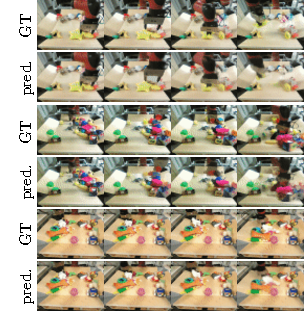
\includegraphics[width=.8\columnwidth,trim={3.2mm 0 0 0},clip]{images_rfr/video_prediction.pdf}
\caption{\small{\todo{Overview of visual MPC concept}}}
\label{fig:video_prediction}
\end{figure}
%%SL.09.03: the figure looks awkwardly stretched, and it's not clear what the robot is actually doing

%Despite the benefits, a number of challenges arise when aiming to use sensory prediction models: how can we learn a model of high-dimensional observations, and how should an objective or reward be determined with respect to the predicted observations? %how should experience be collected? %how should actions be chosen with respect to the model?
%We discuss each of these design decisions and propose several options, weighting the benefits and trade-offs of each.
%%SL.09.03: sounds a bit too much like a laundry list, can we pull some broader themes and dive into details later?
%Our overall approach amounts to a deep model-based reinforcement learning algorithm that leverages video prediction models to achieve a variety of pixel-based control tasks without shaped reward information.

The main contributions of this work are as follows. We propose a general framework for deep reinforcement learning with sensory prediction models that is suitable for learning behaviors in diverse, open-world environments with minimal reward feedback. 
%FE.10.13:Same thing with the reward here...
We present model architectures that are effective for predicting pixel-level observations amid occlusions and novel objects. Unlike low-dimensional representations of state, specifying and evaluating the reward from pixel predictions is nontrivial: we present several practical methods for specifying and evaluating progress towards the goal---including distances to goal pixel positions, registration to goal images, and image classifiers---and compare their effectiveness and use-cases.
%, abstracting away the model architecture %, the policy optimization, 
%and the form of the reward function with respect to predicted observations.
%%SL.09.03: seems reasonable, but when we abstract away so much, we just get the classic model-based RL problem setting. Maybe this is a little bit too much abstraction.
%We then propose model architectures for prediction that can better maintain object permanence through occlusions via temporal skip connections. 
%To handle the challenge of evaluating progress towards the goal from pixel-level predictions, we present several forms of reward specification and evaluation,
%%SL.09.03: I wouldn't put this "Second" -- maybe something more general like architectures for prediction?
%Third, we discuss several forms of planning objectives, 
%including goal pixel positions, goal image registration, and image classifiers.
%%SL.09.03: without motivation, this seems a bit arbitrary. I think this is a good contribution, but the phrasing makes it seem like a less significant detail somehow.
Finally, our evaluation demonstrates that these components can be combined to enable a real robot to perform a range of object manipulation tasks from raw pixel observations. Our experiments include manipulation of previously unseen objects, handling multiple objects, pushing objects around obstructions, handling clutter, recovering from large perturbations, and grasping and maneuvering objects to user-specified locations in 3D-space. These results represent a significant advance in the \emph{generality} of skills that can be acquired by a real robot operating on raw pixel values.

This paper builds upon prior conference papers~\cite{foresight,sna,ebert2018robustness,flo}, presenting them in a unified view; our new contributions include an empirical evaluation of cloth manipulation and placing-based tasks, analysis of each method involving XX, as well as a comprehensive, open-sourced simulation environment to facilitate future research and better reproducibility.


\todo{make big VMPC diagramm!!}



 





